\section{Simulation Results}
The designed converter topology is simulated in Simulink to verify desired functioning of the circuit.

For simplicity, the controller topology and feedback mechanisms are not included in the circuit schematic of the simulation model. Furthermore, the semiconductor devices and filter capacitors and inductors are taken ideal without voltage drops and ESR values.

In order to verify the operation of the circuit, we simulated the converter at its two extreme boundary points for input voltage of $ V_{in} = 24\;V $ and $ V_{in} = 48\;V $.

The Simulink simulation model of the Flyback Converter circuit is given in Figure \ref{fig:schematic}.

\begin{figure}[H]
\begin{center}
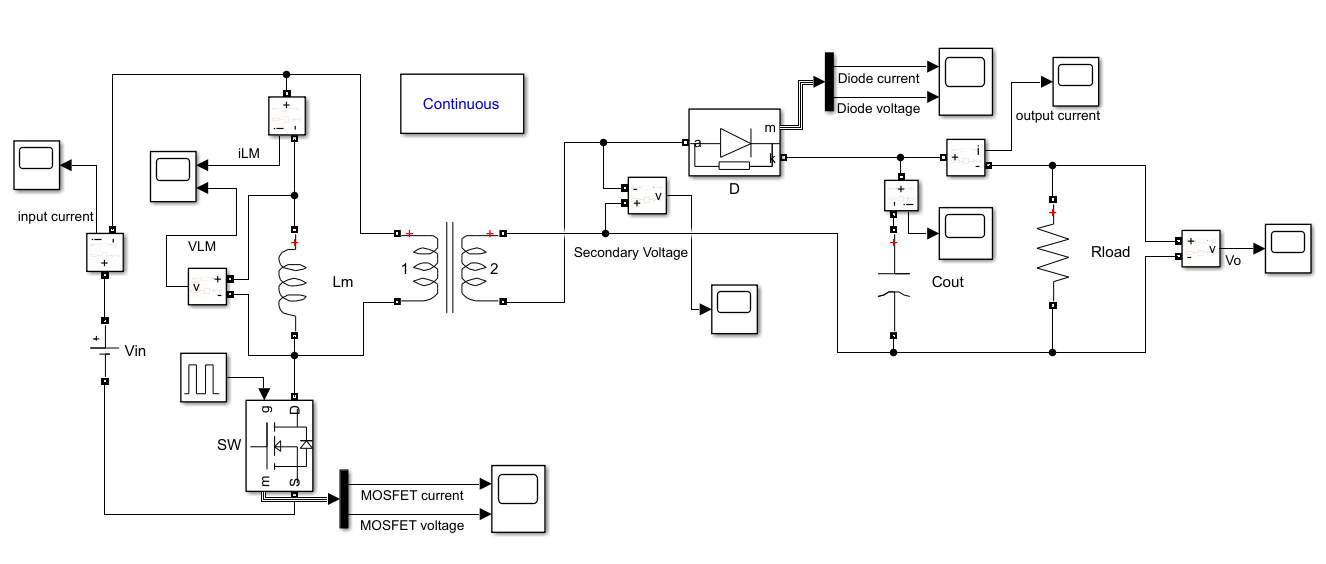
\includegraphics[width=1\textwidth]{schematic.png}
\caption{Simulink Circuit Schematic of the Flyback Converter}
\label{fig:schematic}
\end{center}
\end{figure}

\subsection{Simulation Results for $ V_{in} = 24\;V $}

The simulation results of the converter circuit for input voltage of $ V_{in} = 24\;V $ are given below.

The duty cycle of the MOSFET is determined as $ D = 5\% $ for this operation in order to keep the average output voltage at 15 V.

The duty cycle of the MOSFET is determined by some trial and errors since the converter circuit is operating in DCM. In DCM operation, the standard voltage gain equation can no more be utilized to determine the duty ratio.

The input current waveform of the converter circuit is given in Figure \ref{fig:incurr24}.

\begin{figure}[H]
\begin{center}
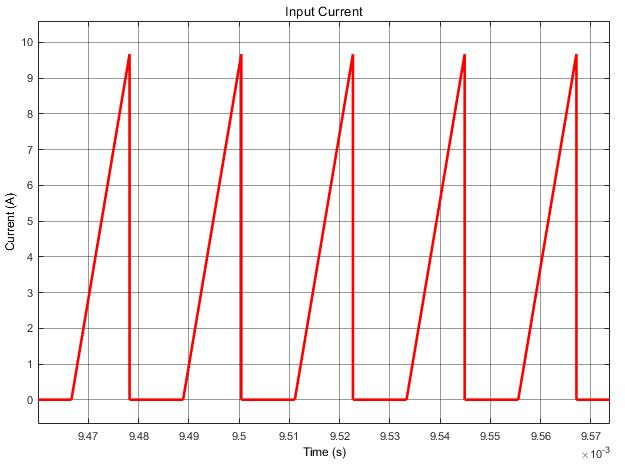
\includegraphics[width=1\textwidth]{input_current_24.jpg}
\caption{Input Current Waveform of the Flyback Converter for $ V_{in} = 24\;V $}
\label{fig:incurr24}
\end{center}
\end{figure}

The input current ripple is high as can be seen from Figure \ref{fig:incurr24} since the switch is positioned in series to the input side. The maximum current drawn from the input source and the peak to peak input current ripple is equal to 9.681 A. The high input current ripple might cause EMI effects by affecting the operation of the analog controller and gate driver circuit of the switch.

The MOSFET current and voltage waveforms of the converter circuit are given in Figure \ref{fig:mos24}.

\begin{figure}[H]
\begin{center}
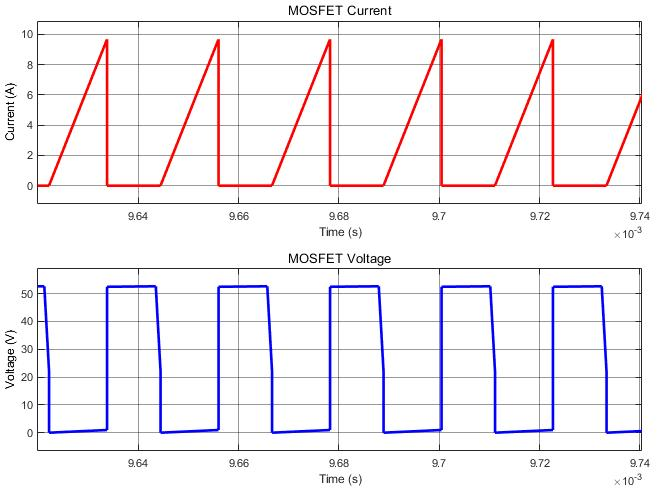
\includegraphics[width=1\textwidth]{MOSFET_curr_volt_24.jpg}
\caption{MOSFET Current and Voltage Waveforms of the Flyback Converter for $ V_{in} = 24\;V $}
\label{fig:mos24}
\end{center}
\end{figure}

The maximum current through the MOSFET during its on period is observed from Figure \ref{fig:mos24} to be 9.681 A. The maximum voltage across the switch during its off period is also observed to be 52.63 V.

The voltage and current waveforms of the magnetizing inductor of the transformer of the converter circuit are given in Figure \ref{fig:ind24}.

\begin{figure}[H]
\begin{center}
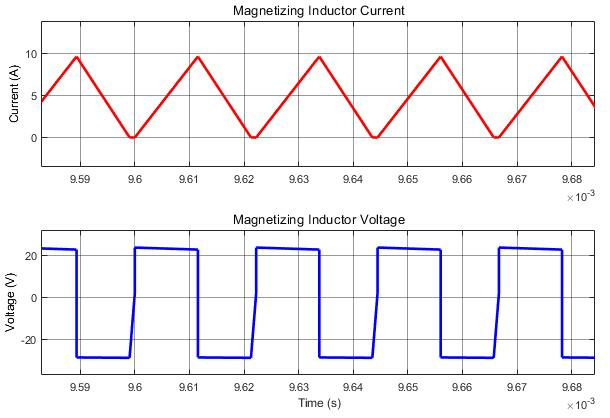
\includegraphics[width=1\textwidth]{inductor_volt_curr_24.jpg}
\caption{Magnetizing Inductor Voltage and Current Waveforms of the Flyback Converter for $ V_{in} = 24\;V $}
\label{fig:ind24}
\end{center}
\end{figure}

The DCM operation of the converter circuit can also be observed from the magnetizing inductor current waveform given in Figure \ref{fig:ind24}. It is seen from the Figure \ref{fig:ind24} that the inductor current reaches to zero and stays at zero for a finite duration until the next switching cycle.

The maximum magnetizing inductor current is observed to be equal to 9.669 A from the simulations.

The magnetizing inductor voltage switches between 24 V and -28.63 V during the switching operation.

The diode voltage and current waveforms of the converter circuit are given in Figure \ref{fig:dio24}.

\begin{figure}[H]
\begin{center}
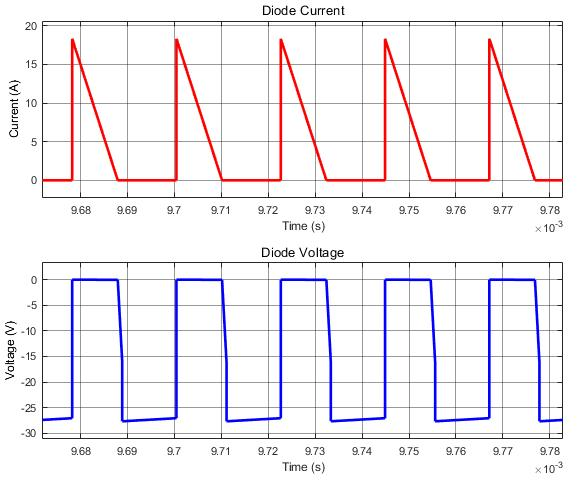
\includegraphics[width=1\textwidth]{diode_curr_volt_24.jpg}
\caption{Diode Voltage and Current Waveforms of the Flyback Converter for $ V_{in} = 24\;V $}
\label{fig:dio24}
\end{center}
\end{figure}

The voltage waveform on the secondary side of the transformer of the converter circuit is given in Figure \ref{sec24}.

\begin{figure}[H]
\begin{center}
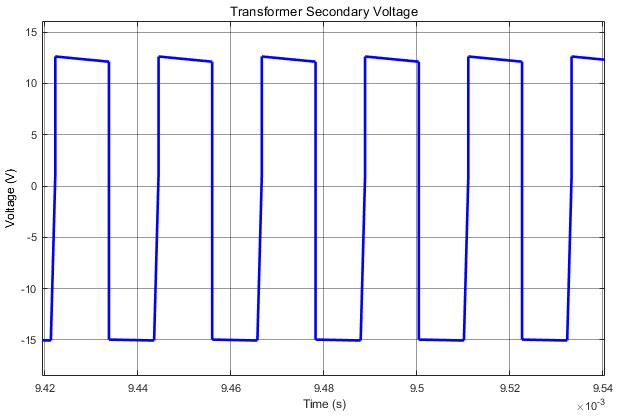
\includegraphics[width=1\textwidth]{secondary_voltage_24.jpg}
\caption{Secondary Voltage Waveform of the Transformer of the Flyback Converter for $ V_{in} = 24\;V $}
\label{fig:sec24}
\end{center}
\end{figure}

The secondary side voltage of the transformer switches between 12.63 V and -15 V during the switching operation.

The output current waveform of the converter circuit is given in Figure \ref{fig:outcurr24}.

\begin{figure}[H]
\begin{center}
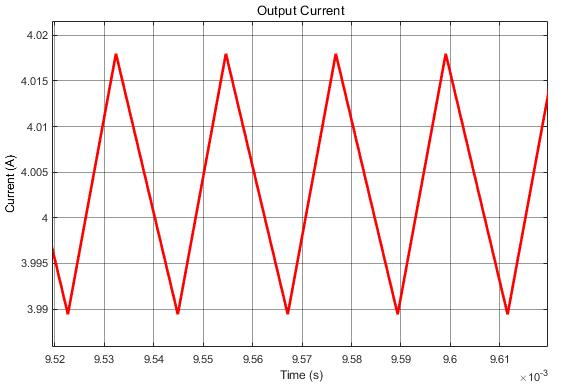
\includegraphics[width=1\textwidth]{output_current_24.jpg}
\caption{Output Current Waveform of the Flyback Converter for $ V_{in} = 24\;V $}
\label{fig:outcurr24}
\end{center}
\end{figure}

The average output current is approximately obtained as 4 A.

The output voltage waveform of the converter circuit is given in Figure \ref{fig:outvolt24}.

\begin{figure}[H]
\begin{center}
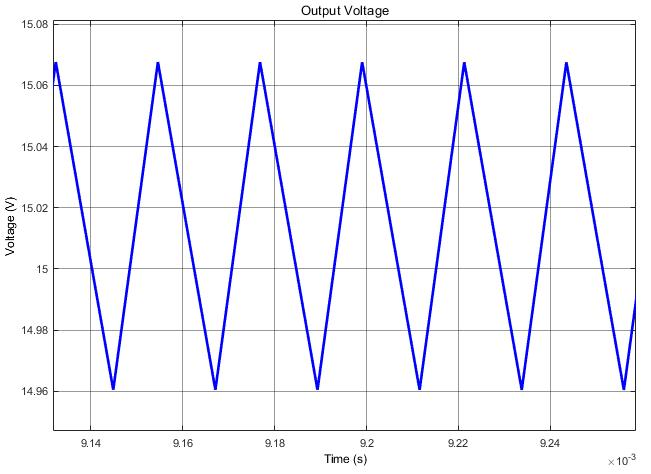
\includegraphics[width=1\textwidth]{output_voltage_24.jpg}
\caption{Output Voltage Waveform of the Flyback Converter for $ V_{in} = 24\;V $}
\label{fig:outvolt24}
\end{center}
\end{figure}

The average output voltage is obtained as 15 V as can be seen from Figure \ref{fig:outvolt24}. The peak to peak output voltage ripple is approximately equal to 0.116 V, which is less than the desired peak to peak output voltage ripple limit (4\%) of 0.6 V.

\subsection{Simulation Results for $ V_{in} = 48\;V $}

The simulation results of the converter circuit for input voltage of $ V_{in} = 48\;V $ are given below.

The duty cycle of the MOSFET is determined as $ D = 0.52\% $ for this operation in order to keep the average output voltage at 15 V.

The input current waveform of the converter circuit is given in Figure \ref{fig:incurr48}.

\begin{figure}[H]
\begin{center}
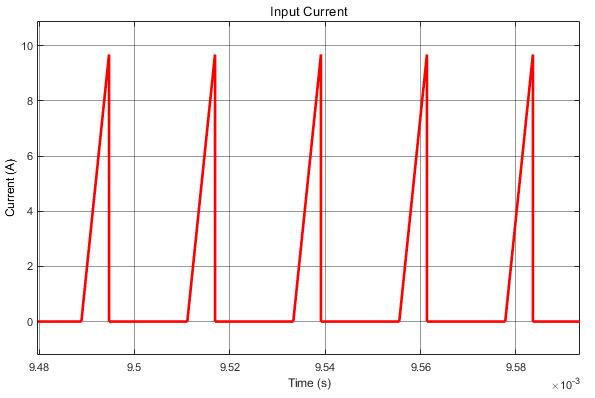
\includegraphics[width=1\textwidth]{input_current_48.jpg}
\caption{Input Current Waveform of the Flyback Converter for $ V_{in} = 48\;V $}
\label{fig:incurr48}
\end{center}
\end{figure}

Similar to the previous condition, the input current ripple is high as can be seen from Figure \ref{fig:incurr48} since the switch is positioned in series to the input side. The maximum current drawn from the input source and the peak to peak input current ripple is equal to 9.690 A. The high input current ripple might cause EMI effects by affecting the operation of the analog controller and gate driver circuit of the switch.

The MOSFET current and voltage waveforms of the converter circuit are given in Figure \ref{fig:mos48}.

\begin{figure}[H]
\begin{center}
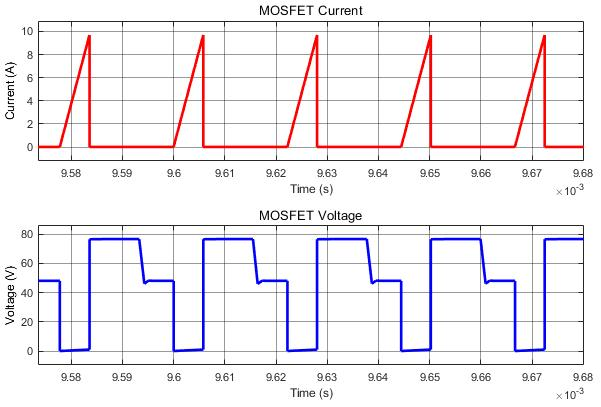
\includegraphics[width=1\textwidth]{MOSFET_curr_volt_48.jpg}
\caption{MOSFET Current and Voltage Waveforms of the Flyback Converter for $ V_{in} = 48\;V $}
\label{fig:mos48}
\end{center}
\end{figure}

The maximum current through the MOSFET during its on period is observed from Figure \ref{fig:mos48} to be 9.690 A. The maximum voltage across the switch during its off period is also observed to be 76.63 V.

It is also possible to clearly observe the DCM operation of the converter circuit from the MOSFET voltage waveform given in Figure \ref{fig:mos48}. During the off period of the switch, the voltage across the MOSFET is equal to 76.63 V until the magnetizing inductor current becomes zero. Then, until the next switching cycle (until the MOSFET becomes on again), the MOSFET voltage drops down to the input voltage ($ V_{MOSFET} = 48\;V $) and stays at this level.

The voltage and current waveforms of the magnetizing inductor of the transformer of the converter circuit are given in Figure \ref{fig:ind48}.

\begin{figure}[H]
\begin{center}
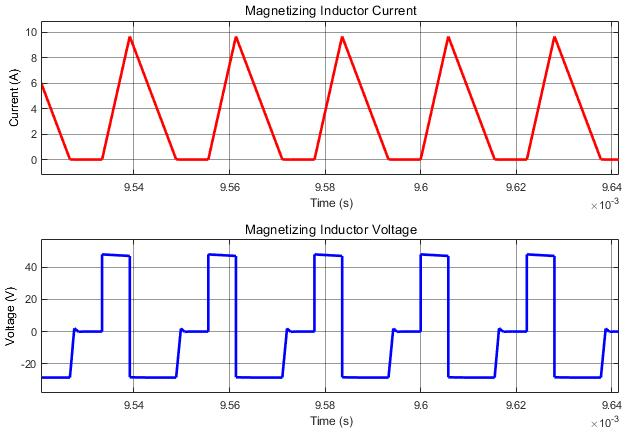
\includegraphics[width=1\textwidth]{inductor_curr_volt_48.jpg}
\caption{Magnetizing Inductor Voltage and Current Waveforms of the Flyback Converter for $ V_{in} = 48\;V $}
\label{fig:ind48}
\end{center}
\end{figure}

Again, it is also possible to observe the DCM operation from the magnetizing inductor current and voltage waveforms given in Figure \ref{fig:ind48}.

The maximum magnetizing inductor current for this operation is observed to be equal to 9.664 A.

The magnetizing inductor current discharges through the transformer and reaches to zero during the off period of the switch, and stays zero until the next switching cycle (until the MOSFET becomes on again). The magnetizing inductor voltage during that process changes from -28.63 V to 0 V when the inductor current becomes zero. During the on period of the switch, the magnetizing inductor voltage is equal to the input voltage ($ V_{inductor} = 48\;V $), and the magnetizing inductor charges linearly.

The diode voltage and current waveforms of the converter circuit are given in Figure \ref{fig:dio48}.

\begin{figure}[H]
\begin{center}
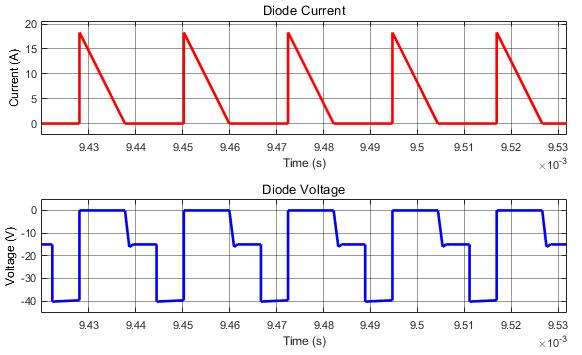
\includegraphics[width=1\textwidth]{diode_curr_volt_48.jpg}
\caption{Diode Voltage and Current Waveforms of the Flyback Converter for $ V_{in} = 48\;V $}
\label{fig:dio48}
\end{center}
\end{figure}

The DCM operation can also be clearly observed from the diode voltage waveform given in Figure \ref{fig:dio48}. During the off period of the switch, the diode stays on until the magnetizing inductor current becomes zero. Then, the diode becomes off, and stays off until the next off period of the switch. The reverse voltage across the diode during its off period changes from -15 V to -40.263 V due to this DCM operation. 

The voltage waveform on the secondary side of the transformer of the converter circuit is given in Figure \ref{sec48}.

\begin{figure}[H]
\begin{center}
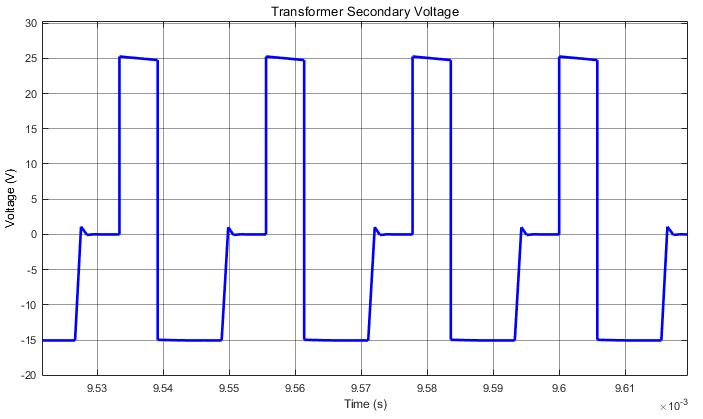
\includegraphics[width=1\textwidth]{secondary_voltage_48.jpg}
\caption{Secondary Voltage Waveform of the Transformer of the Flyback Converter for $ V_{in} = 48\;V $}
\label{fig:sec48}
\end{center}
\end{figure}

Similarly, the secondary side voltage of the transformer also exhibits some DCM behavior. During the off period of the switch, the secondary voltage is equal to the negative of the output voltage ($ V_{sec} = -15\;V $) until the magnetizing inductor current becomes zero. When the magnetizing inductor current becomes zero, the diode at the output side switches off and the secondary side voltage becomes zero.

During the on period of the switch, the magnetizing inductor charges from input. Hence, the voltage across the primary side of the transformer is equal to the input voltage ($V_{pri} = 48\;V $). As a result, the secondary side voltage becomes 25.263 V during that period due to the turn ratio between the primary and the secondary.


The output current waveform of the converter circuit is given in Figure \ref{fig:outcurr48}.

\begin{figure}[H]
\begin{center}
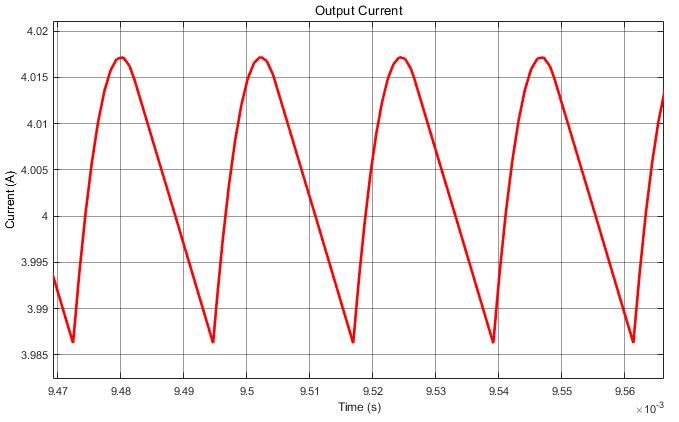
\includegraphics[width=1\textwidth]{output_current_48.jpg}
\caption{Output Current Waveform of the Flyback Converter for $ V_{in} = 48\;V $}
\label{fig:outcurr48}
\end{center}
\end{figure}

As seen from Figure \ref{fig:outcurr48} output current waveform is between 3.987 and 4.017. This current ripple is good enough for Flyback Converter. There is only resistive load, so output ripple current must be smaller than 0.15 A. In this simulation results, output current ripple is 0.03 A which is less than 0.15 Ampere.

The output voltage waveform of the converter circuit is given in Figure \ref{fig:outvolt48}.


\begin{figure}[H]
\begin{center}
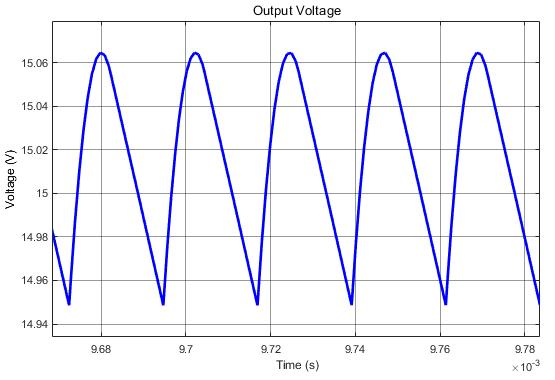
\includegraphics[width=1\textwidth]{output_voltage_48.jpg}
\caption{Output Voltage Waveform of the Flyback Converter for $ V_{in} = 48\;V $}
\label{fig:outvolt48}
\end{center}
\end{figure}

As seen from Figure \ref{fig:outvolt48}. output voltage waveform is between 15.06 and 14.96 V. Expected output voltage of e design is 15 V and output voltage ripple limit is 0.6 V. $15.06-14.96=0.1 v$ is below the design specification limits. This output voltage ripple  depends on output capacitor. 470 $\mu$F capacitor was used in simulations. Average output voltage is 15 V as expected. There is resistive load on the flyback converter thats why the shape of the output voltage is similar to the output current. Actually output voltage waveform is 3.75 times output current waveform. Output voltage waveform for 48 V input should be similar with output voltage waveform but there is differences due to different time intervals.